\documentclass[a4paper, 12pt]{article}

\usepackage[utf8]{inputenc} % for UTF-8 support
\usepackage{graphicx} % for images

\graphicspath{ {./images/} } % put images in here

\title{AI for IMGD Final Project Report}
\author{Cole Granof \and Joseph Petitti \and Matthew Puentes}
\date{\today}

\begin{document}

\maketitle

\section{What We Did}

For the final AI for IMGD project we created a procedurally generated, top-down,
twin stick shooter game, inspired by games like \textit{The Binding of Isaac}
and \textit{Nuclear Throne}. In the game, the player controls a small
eyeball-like character that can move around the game world, a large series of
caves. There are several types of enemies that inhabit the caves, including some
that chase the player, others that wander around randomly, and even some that
can shoot bullets. Players fight these enemies while exploring the cave to track
down three Boss enemies, which must be defeated to win. They can also find power
ups hidden the caves, powerful artifacts that increase the player's abilities in
unique ways.

The hero is controlled with a keyboard or gamepad, and can move around and shoot
in any direction. Like all game entities in our custom engine, the hero has a
velocity, acceleration, and drag. This allows it realistically reach a maximum
speed in a way that is simple to program and maintain.

There are three main enemy types: Chase, Scatter, and Shooter. Chase enemies
sleep until the player comes close or shoots at them, but chase after the hero
as soon as they wake up. Scatter enemies wander around the board in random and
unpredictable ways. Shooter enemies maintain their distance and fire slow-moving
projectiles at the hero. Each enemy has a random chance to be bigger. Bigger
enemies split into several smaller enemies when they are killed, providing
varying levels of difficulty.

Each enemy type has a different type of face, which is further modified by
randomly generated parameters. For example, Chase enemies have one large eye in
the center of their face, but the size and positioning of their eye and mouth is
tweaked by parameters. The game world has randomly generated color scheme, which
is applied to the cave environment as well as enemies.

The game also features a robust power up system. All power ups are applicable to
both the hero and the enemies---both are abstracted to a Creature superclass.
All Creatures share functionality such as speed, shot rate, and bullet damage.
In this way, it's easy to create unique and challenging enemies by applying
randomized power ups to them. We plan to eventually have 26 different power
ups (one for each letter of the alphabet), but for this early beta version we
have only seven.

To make our game accessible to as many people as possible we implemented it in
JavaScript using the HTML5 canvas API for graphics. To give ourselves the most
control over the game environment we decided to write absolutely everything
ourselves, from scratch. We use no game engine, no third party libraries, no
preprocessor, no front-end build tools, and no graphics API but the one built in
to every browser. We implemented a full-fledged game engine in JavaScript that
runs game logic independent of screen refresh rate, handles collisions in an
efficient way, has a robust collision-mapping system using first-class
functions, implements basic kinematics and particles, has customizable camera
controls, and uses generalized keyboard and gamepad input.

\section{Why We Did It}

% TODO write

\section{How It Relates to Things We Read}

% TODO write

\section{How It Works}

Caves are generated with an augmented rule set of Conway's Game of Life. Instead
of the typical rules, a cell dies if it has anywhere from zero to three
neighbors. A cell stays the same if it has 4 neighbors. If a cell has greater
than four neighbors, a new cell is born. Unlike Conway's Game of Life, this
rule set reaches a stable state after only a few iterations, and produces the
cave-like structures you see in our game. We also count cells that are outside
the boundary of the grid as alive cells. Figures

First, we randomize the initial state of our board. In our game, a cell has
about a fifty percent chance of being alive. Then, we run this augmented Game of
Life for twenty generates. The end state of this simulation is the basis for our
level layout. Figures~\ref{fig:initialCave}-\ref{fig:finalCave} in
Section~\ref{sec:cavePictures} shows the result of the algorithm in action.

The one drawback of using cellular automata is that they are chaotic; it is very
hard to choose initial conditions to create a specific outcome. Because of this,
we often do not end up with a cave-system that is fully traversable. To overcome
this, we search the grid to identify each unique cave. We mark the largest cave
as the ``main cave'' and connect each ``sub cave'' to the main cave with a
tunnel of destroyable blocks.

Because we have knowledge of the size of each cave that is generated, we use
this to make our power-ups spawn in more interesting locations. Small caves have
a high density of power-ups, making them loot caches which are fun to find. This
encourages the player to explore the map and find the small caves that spawn.
Effectively, the chance for a power-up to spawn is inversely proportional to the
size of the cave.


% TODO write

\section{Evaluation Results}

% TODO write


\section{What Those Results Mean}

% TODO write


\section{What We Learned}

% TODO write


\section{Self Evaluation}

\subsection{Cole Granof}

I worked on implementing game engine features so that my teammates would be able
to easily add functionality to our game. This included a particle system, basic
kinematics, and a system from adding behaviors to entities in the world. This
was a lot of work to do without any external libraries, but I am happy with the
result.

Throughout the development, I added various optimizations so that we could have
larger worlds with more enemies, all with minimal to no slowdown.

I took the first pass at generating random cave levels using cellular automata.
Matt improved on this by connecting the disconnected caves with breakable walls
so that the entire cave was traversable.


\section{Cave Pictures}
\label{sec:cavePictures}

\begin{figure}[h]
	\centering
	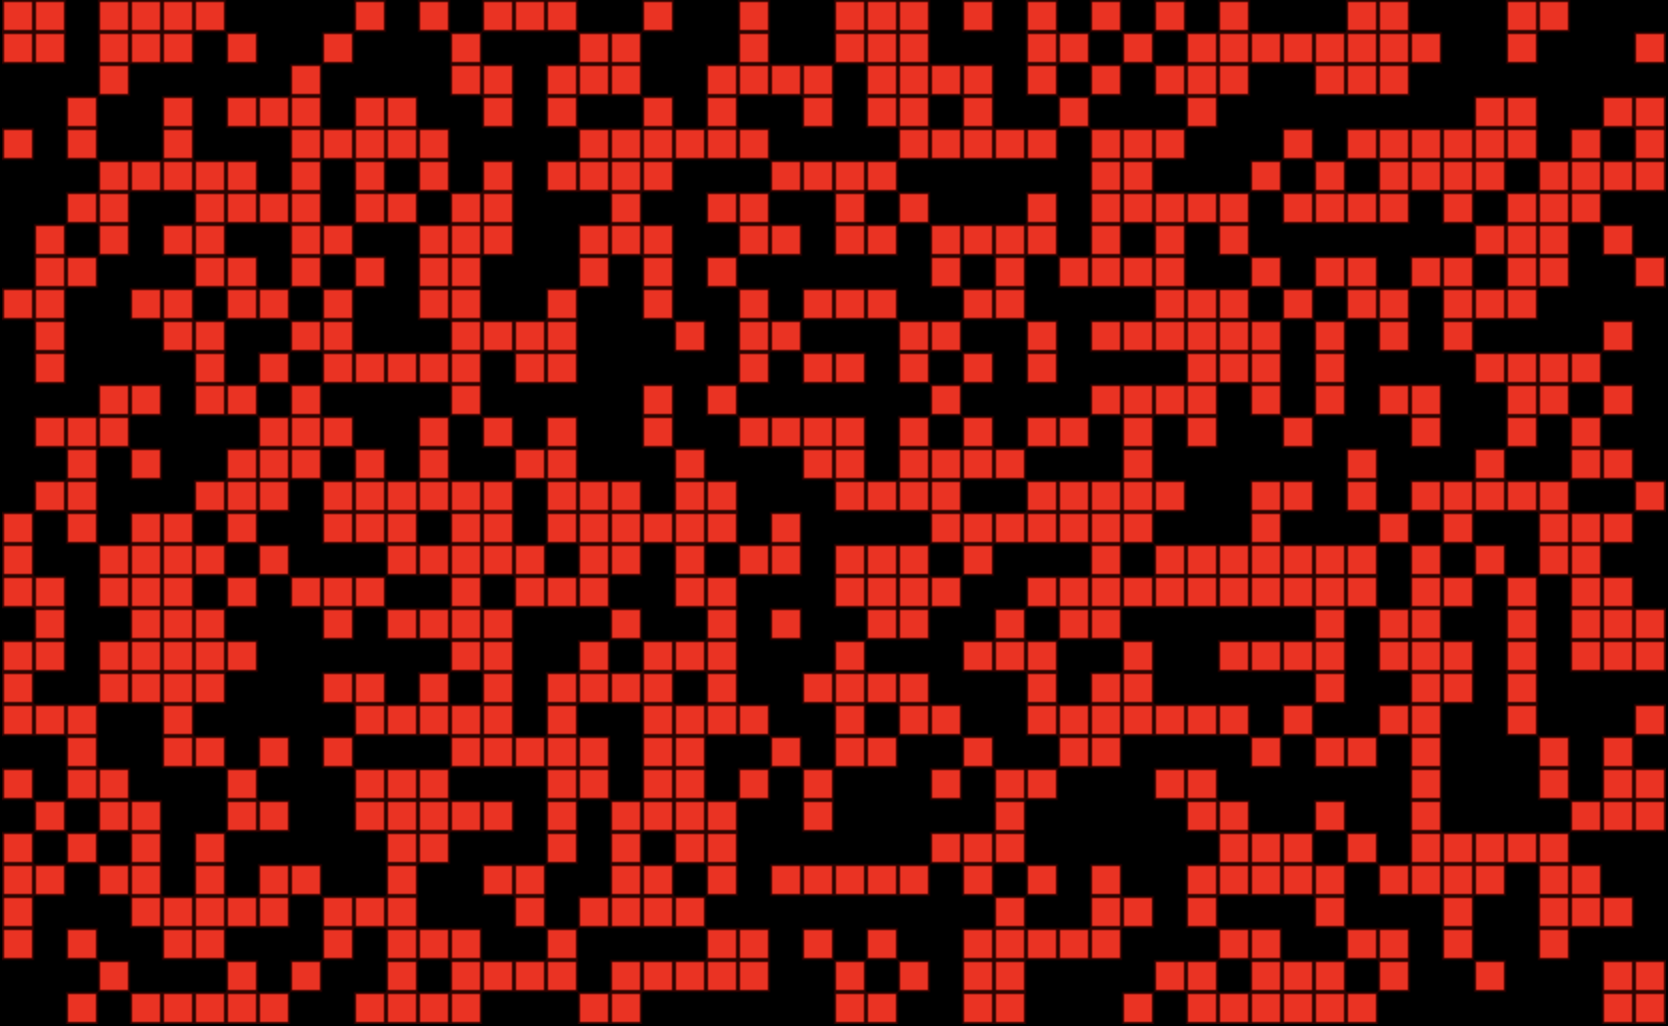
\includegraphics[width=\textwidth]{initial-cave.png}
	\caption{The initial cave on a randomized board}
	\label{fig:initialCave}
\end{figure}

\begin{figure}[h]
	\centering
	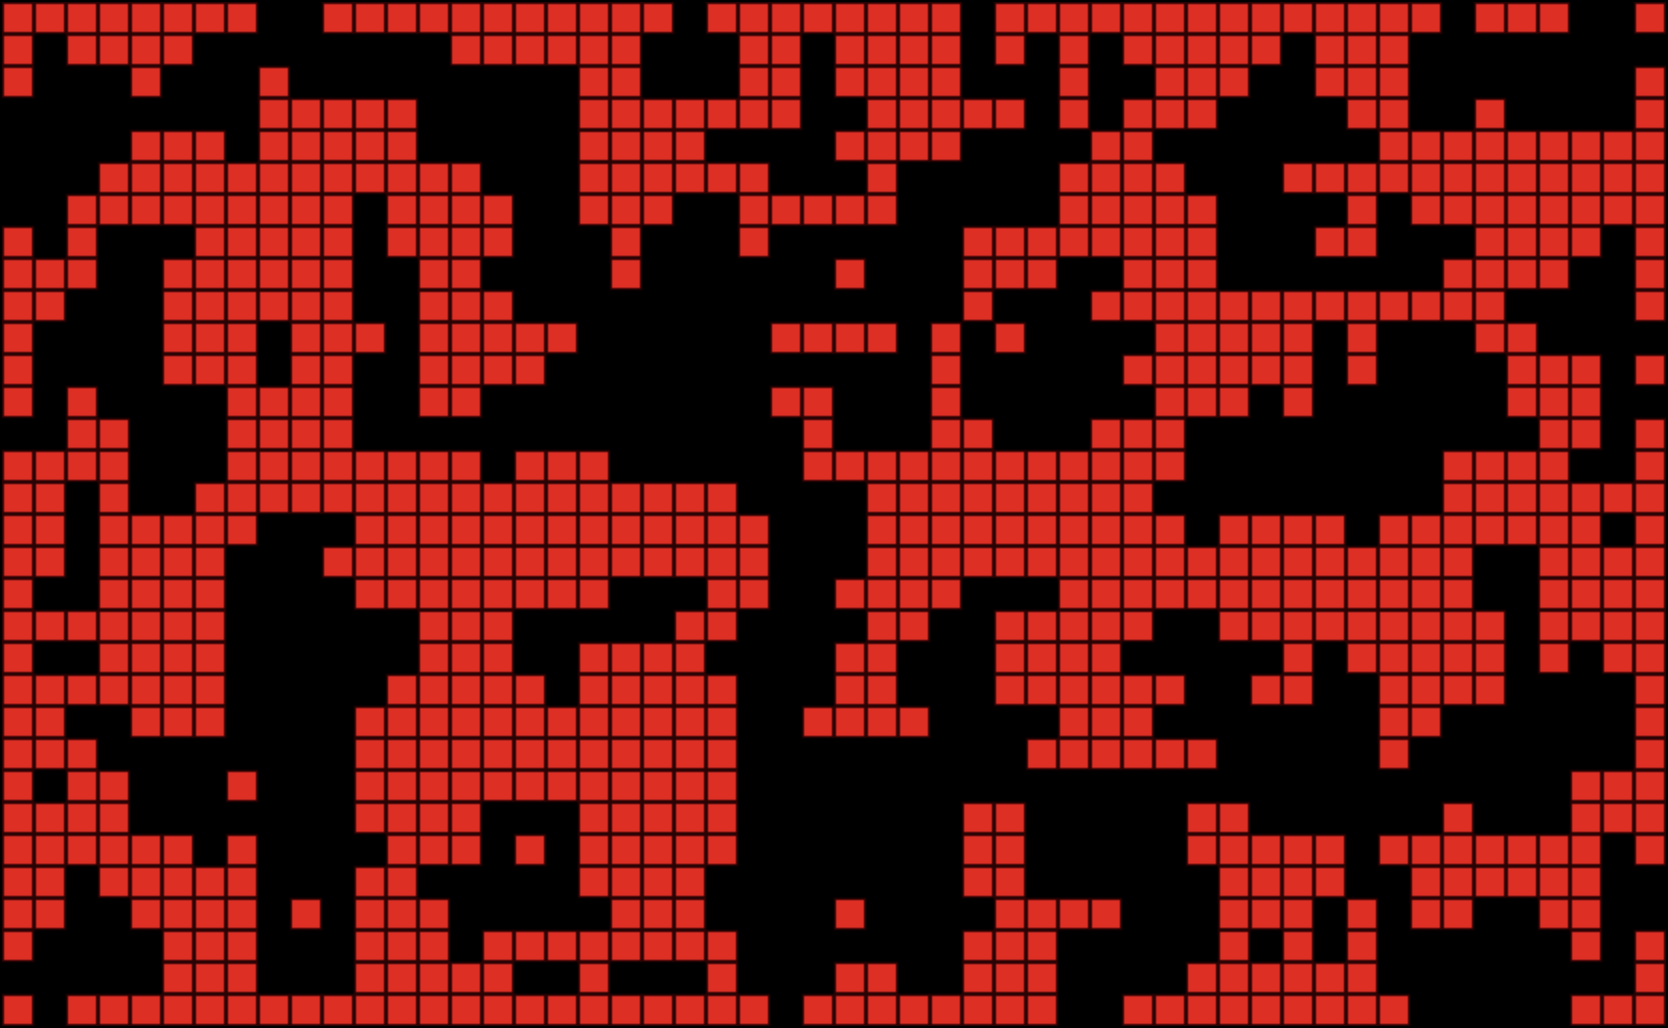
\includegraphics[width=\textwidth]{one-step-cave.png}
	\caption{The final cave after reaching a steady state}
	\label{fig:oneStepCave}
\end{figure}

\begin{figure}[h]
	\centering
	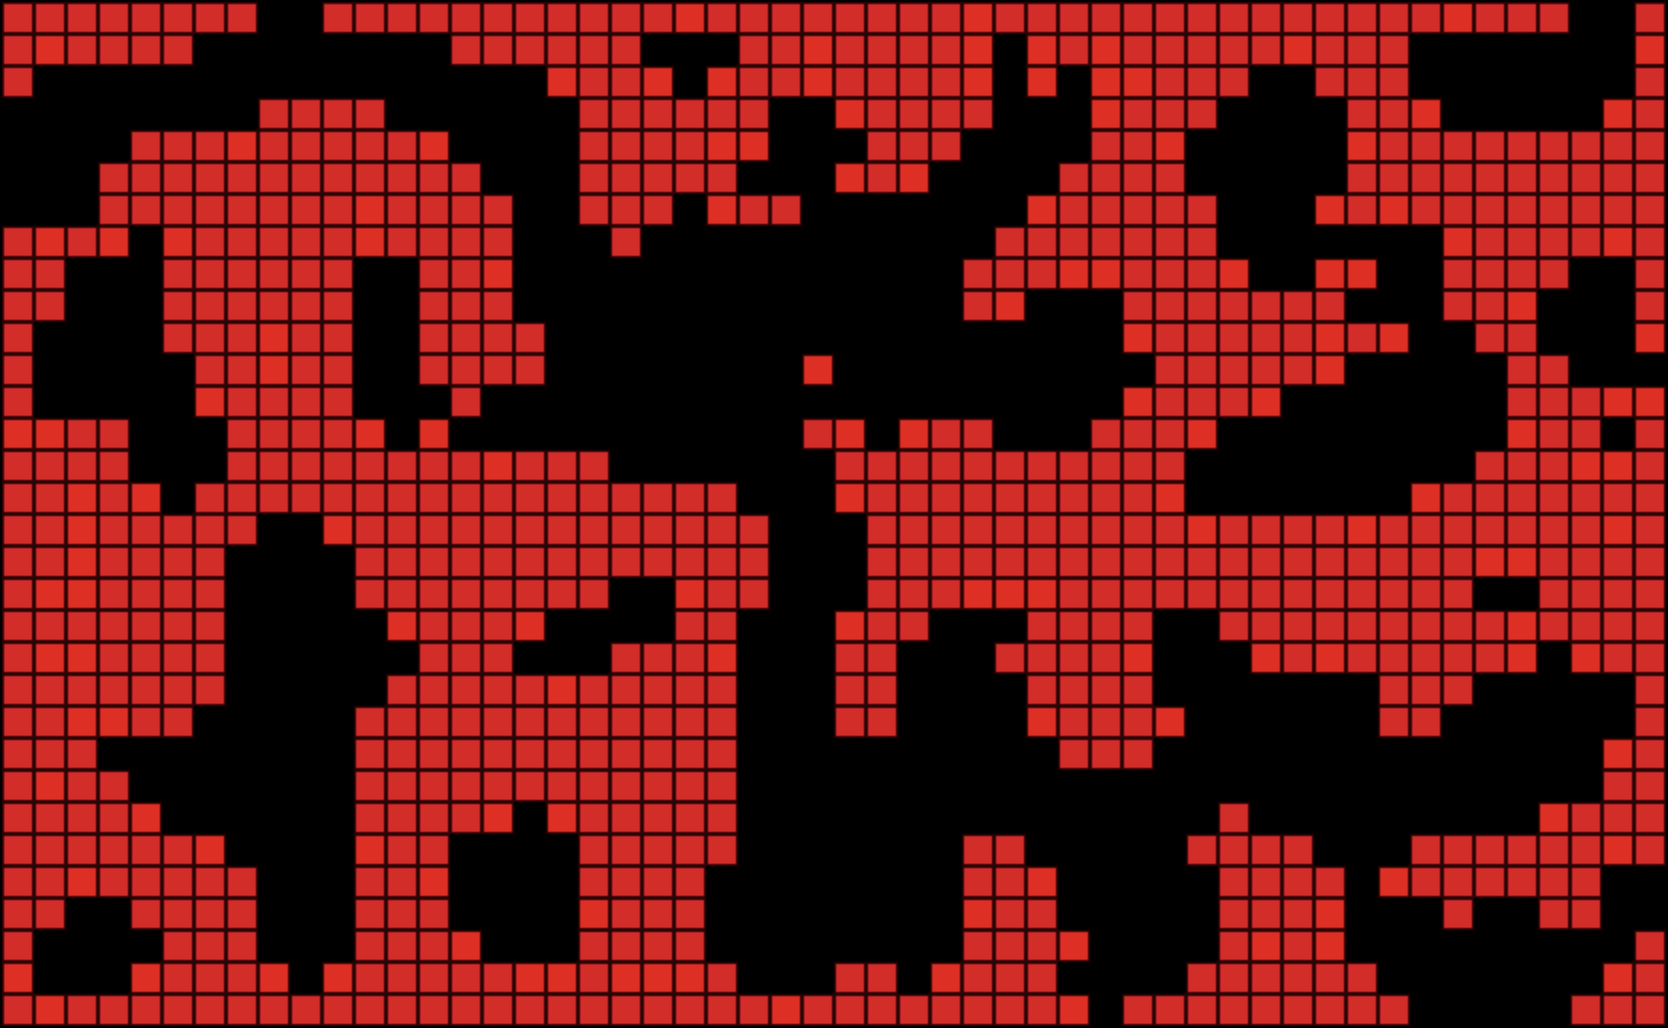
\includegraphics[width=\textwidth]{two-step-cave.png}
	\caption{The cave after two steps}
	\label{fig:twoStepCave}
\end{figure}

\begin{figure}[h]
	\centering
	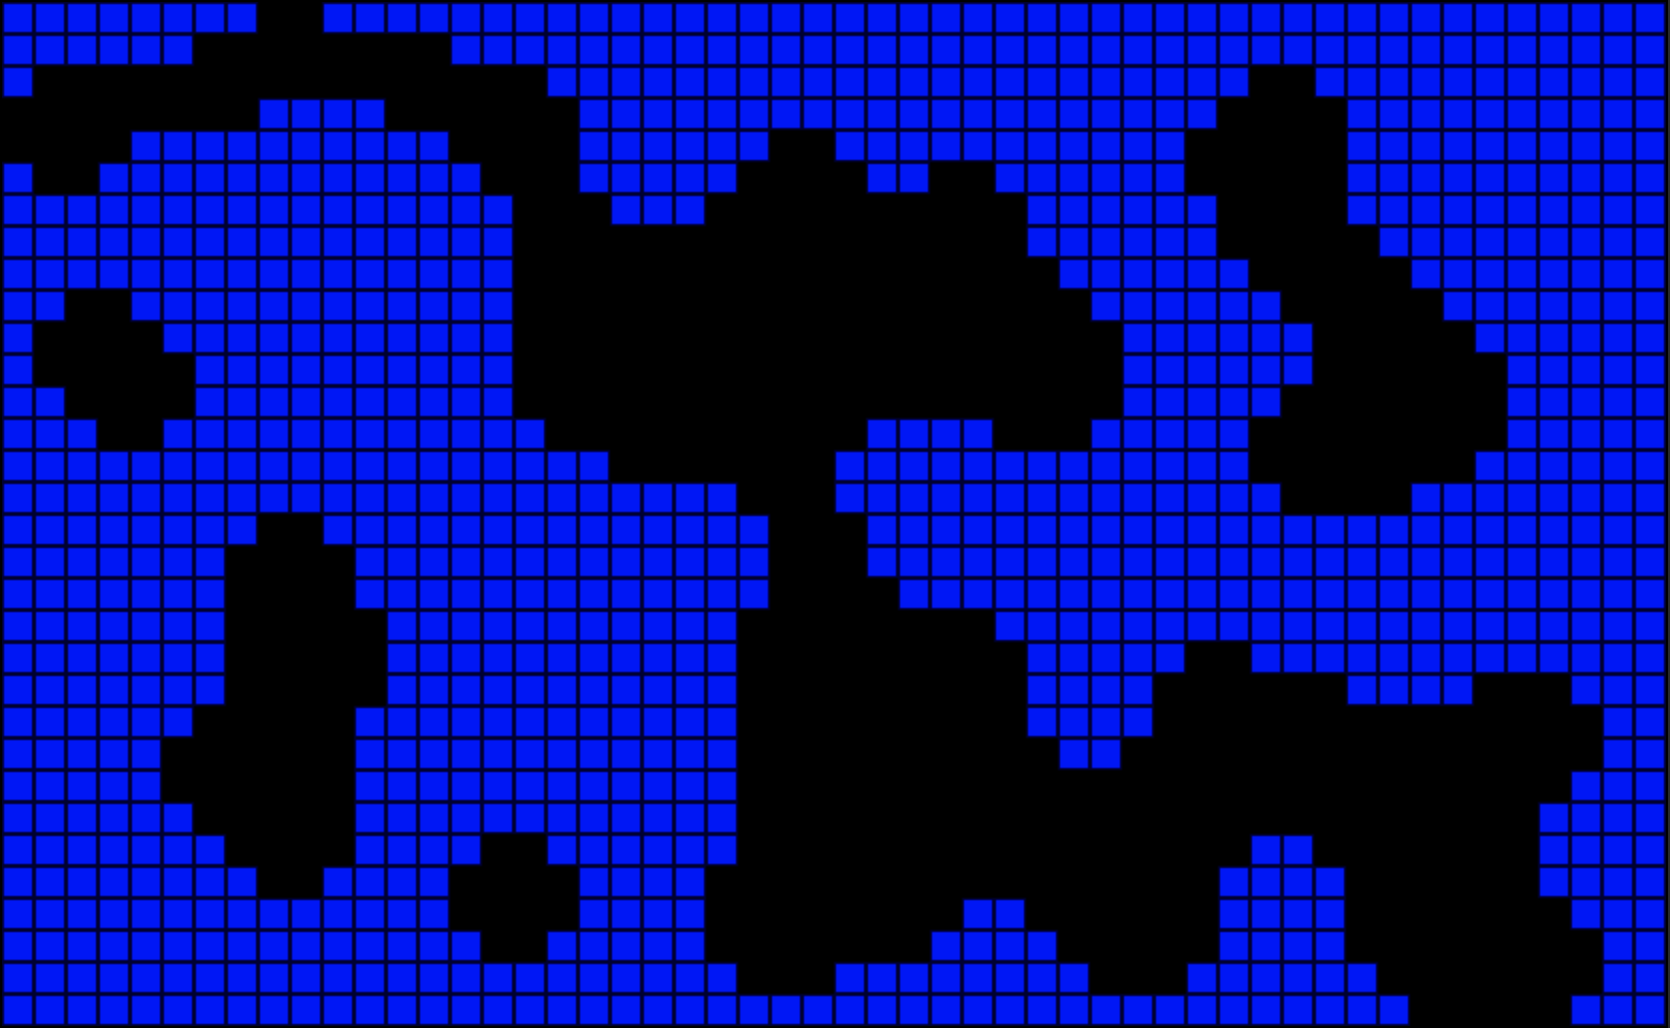
\includegraphics[width=\textwidth]{final-cave.png}
	\caption{The final cave after reaching a steady state}
	\label{fig:finalCave}
\end{figure}


\end{document}

